\documentclass[11pt,a4paper]{article}
\usepackage[utf8]{inputenc}
\usepackage[margin=2cm]{geometry}
\usepackage{bm} % for bold maths symbols
\usepackage{enumitem} % for more flexibility with lists
\usepackage{array}  % to give vertical centering in tables
\usepackage[pdftex]{graphicx} % for including images
\usepackage{subcaption} % for side by side figures
\usepackage{amssymb} % for mathbb
\usepackage{amsmath} % for align and tfrac
\usepackage{amsthm} % for theorem / proofs
\usepackage{natbib}
\usepackage{hyperref} % for interactable links
\usepackage{authblk} % for author and affiliations
\usepackage{fancyhdr} % For headers and footers
\usepackage{tikz-cd}
\bibliographystyle{plainnat}
\usepackage{lineno}

% Some common commands used by Tom
\newcommand{\grad}[1]{{\bm{\nabla}{#1}}}
\newcommand{\dv}[1]{\bm{\nabla\cdot{#1}}}
\newcommand{\curl}[1]{\bm{\nabla}\times\bm{#1}}
\newcommand{\pfrac}[2]{\frac{\partial{#1}}{\partial{#2}}}
\newcommand{\dx}[1]{\hspace{0.75mm}\mathrm{d}{#1}}
\newcommand{\der}[2]{\frac{\dx{#1}}{\dx{#2}}}
\newcommand{\cder}[2]{\frac{\mathrm{D}#1}{\mathrm{D}#2}}
\newcommand{\curlybrackets}[1]{\left\lbrace{#1}\right\rbrace}

\newtheorem{requirement}{Requirement}
\newtheorem{theorem}{Theorem}
\newtheorem{lemma}{Lemma}
\newtheorem{proposition}{Proposition}

% --------------------------------------------------- %
% Things depending on where this is being submitted
% --------------------------------------------------- %
% Header / Footer for adding Crown copyright statement
\pagestyle{fancy}
\fancyhf{}
% \lfoot{\textcopyright \ Crown Copyright, Met Office}
\cfoot{\thepage}

% Need to adjust it for the first page as well
\fancypagestyle{plain}{
\fancyhf{}
% \lfoot{\textcopyright \ Crown Copyright, Met Office}
\cfoot{\thepage}
}



\begin{document}

\section*{Authors' Response To Referees' Comments}
We would like to greatly thank the referees for the time and efforts spent in reviewing our manuscript, and for their helpful comments.
We have provided a ``tracked changes'' version of the manuscript, with amendments highlighted in red where possible.
\\
\\
The most significant changes that we have made are:
\begin{itemize}[leftmargin=*]
\item Reorganising Section 2, bringing Section 2(c) part 1 earlier, so that description of 1D schemes now precedes the recap of the COSMIC splitting;
\item Amending the notation used for the flux operators to reduce confusion. This also allows the description of conservative tracer transport to be simplified (and several equations to be removed).
\end{itemize}
We have also made a handful of other amendments to issues that we have noticed since the original submission:
\begin{itemize}
    \item There was an inconsistency in the time that the test cases were run for. This has been corrected.
    \item We have slightly changed which unity fields are used in the 3D transport of density described in part 1 of Section 5(a).
    \item We have corrected minor errors in the equations formerly numbered as (58a) and (62a).
\end{itemize}


\subsection*{Responses to Editor's Comments}
\begin{enumerate}[leftmargin=*]
\item[1.] \textit{The authors should note that the Abstract will be collapsed into a single paragraph by copy editors, in case they want to adjust the text.} \\
\\
\textbf{Response}: Thank you for the suggestion. We have merged the paragraphs but made no other changes here.

\item[2.] \textit{L. 28: please revise the wording, units of speed and time are not directly comparable.} \\
\\
\textbf{Response}: We have made this change.

\item[3.] \textit{L. 34: please edit the text to turn forward references into back references.} \\
\\
\textbf{Response}: We have moved equation (1) forwards in the text.

\item[4.] \textit{L. 92: as mentioned by Reviewer 2, the footnote contains relevant material so it should be best placed in the main text.} \\
\\
\textbf{Response}: We have moved the footnote into the main text in its own paragraph. On reviewing the text, we have now slightly expanded the discussion here to clarify the distinction between Lipschitz numbers calculated at cell centres and at facets.

\item[5.] \textit{L. 300: if section 2c1) contains original material, it may be a good idea to move it to section 3, so section 2 will end up containing a useful recap of available methods, while section 3 will feature the authors' own developments.} \\
\\
\textbf{Response}: Thank you for raising this point -- we have struggled to decide on where to place the content in Section 2c1. When undertaking this work, while we did derive the approach for conservative tracer transport described in that section, we then reviewed Skamarock (2006) and felt that he may have used the same method, but without describing it explicitly. So it wasn't completely clear to us whether the content of that section is novel.
As Reviewer 1 suggests moving this material so that it is adjacent to 2a, we have done that instead. Then the narrative of the paper is:
Section 2 (a) the 1D method for density, Section 2(b) the 1D method for conservative tracers, (c) the Lin-Rood/COSMIC scheme.

\item[6.] \textit{[Figs. 2-5] Using a slash between the field name (or dimension) and units is confusing because it appears to be division.  The authors should use parentheses around units instead.} \\
\\
\textbf{Response}: This has been done.

\item[7.] \textit{L. 745: have the authors checked the convergence properties of the 3D version? These need not be added to the manuscript but it would be helpful to have a confirmation and perhaps a short reference in the text. } \\
\\
\textbf{Response}: We have checked 3D convergence rates and we get similar convergence rates to the two-dimensional tests with varying $\rho$. For small Courant number, we see the convergence rates of $\rho$ to be that of the underlying one-dimensional scheme, 3rd order in this case. Using the limiter reduces the order of the tracer. For large Courant number, both $\rho$ and $m$ converge at approximately second-order due to the second-order splitting error. These results hold for both COSMIC and SWIFT splitting. We plan to include convergence tests of the 3D scheme in our next paper which focuses on a spherical domain.

\item[8.] \textit{L. 818: The last paragraph would be best placed earlier in the conclusion, so the manuscript can end with the perspective on future work.} \\
\\
\textbf{Response}: We have removed the final paragraph as this repeated earlier content from the conclusion. This means we now end with the paragraph discussing future work.

\item[9.] \textit{L. 831: The “plotting scripts” should be placed in a public archive, rather than “on request” as noted in the Availability Statement.} \\
\\
\textbf{Response}: We have made a public Github repository to store these, and have updated the Data Availability statement.

\end{enumerate}

\subsection*{Responses to Referee 1}
\underline{Flux operators} \\
\\
\textit{This manuscript would benefit from very clear definitions of the flux operators $\mathcal{F}$.  The text uses this operator in both a two-argument and three-argument form, and both are defined implicitly.  \\
\\
The two-argument $\mathcal{F}(\rho,u)$ is a one-dimensional mass flux, and its first use in equation (16) seems to implicitly define $\mathcal{F}(\rho,u) = F = F^{int} + F^{frac}$, in turn using equations (13) and (14), such that $\mathcal{F}^{x}(\rho,u)$ evaluated at cell $(i+1/2)$ is $F^x_{i+1/2}$.  This operator is also used in equations (18) and (19) to transport mixing ratios (including the unity field), implying that the departure-point calculations and \\
\\
Interpretation of the three-argument $\mathcal{F}(x,F,\rho)$ is more challenging.  This operator is first specified in section 2c (p15, line 306), but its definition depends on $G^{int}$ and $G^{frac}$ from equations (27) and (28), on pages 17 and 18.  However, even this is not entirely clear.  The text states that the fractional part of $\mathcal{F}(x,F,\rho)$ is ``the reconstruction of $m$ multiplied by the fractional part of $F$", but equation (28) defines the multiplication with respect to the fractional part of $\hat{F}$, which is expressly not the fractional part of $F$ (page 17, line 341). \\
\\
This three-argument operator is also used in $\mathcal{F}(\rho,u,\sigma)$ and $\mathcal{F}(m,u,\sigma)$ forms.  I presume in these cases the flux operator is implicitly acting with respect to an underlying volume flux rather than mass flux, and departure points should be computed according to equation (5) rather than (23). However, if that be the case, then it seems like $\mathcal{F}(s,u,\sigma)$ should be identical to the two-argument $\mathcal{F}(s,u)$ (for generic scalar $s$), but equations (36), (37a-b), and (43) use the forms as if they are distinct.} \\
\\
\textbf{Response}: We have made two significant changes to address this:
\begin{itemize}
    \item The flux operator $\mathcal{F}$ now always has three arguments, so that it is $\mathcal{F}(\rho,u,V)$ for density transport and $\mathcal{F}(m,F,\rho V)$ for conservative tracer transport.
    \item We now use the same equations for both the transport of $\rho$ and $m$ to describe the calculation of departure distances and flux integrals. This allowed the removal of the flux $G$ and several other equations, which we think simplifies the manuscript.
\end{itemize}
We have also clarified the point that the operator $\mathcal{F}^{x}$ evaluated at $x_{i+1/2}$ for the dry density is written as $F^x_{i+1/2}$.
\\
\\
\underline{Organization of the main equations} \\
\\
\textit{I think that the SWIFT results are developed well and thoroughly, but when reading through the manuscript it is difficult to appreciate the differences between the SWIFT and COSMIC schemes without extensive cross-referencing.  It appears that the main differences between COSMIC and SWIFT come by replacing equations (20) and (21) by (32)-(34) and (36) and equations (30) and (31) by (38), (39), and (41).  It would be convenient if these differences existed side-by-side somewhere in the paper (perhaps as a table?), so that someone seeking to implement this scheme can have a handy checklist of what FFSL-based operators need updating. \\
\\
The ``storyline" of these methods is also somewhat lost in the presentation.  It seems to me that the principal difference is that COSMIC acts a bit like a midpoint method, building density and mixing ratios at $\Delta t/2$ through advective transport to use in computation of conservative transport to $\Delta t$, whereas SWIFT acts more like an extrapolated trapezoidal rule by averaging fluxes valid at $t=0$ and $t=\Delta t$.  However, this conclusion is tentatively reached by noting the differences between the equations, rather than something explicitly noted in a motivation or discussion section. \\
\\
It may also be helpful to present the one-dimensional results first and then review the COSMIC splitting and describe the SWIFT method.  As it stands, the organization is: \\
\\
1. One-dimensional departure-point calculations for density (or 'volume mixing ratios', I suppose), 2. One-dimensional flux integrals, with integer and fractional splittings, 3. The one-dimensional advective operator, 4. Two-dimensional COSMIC splitting for density, 5. One-dimensional conservative transport of scalar mass (mass mixing ratios), 6. Two-dimensional COMSIC splitting for tracers, and finally 7. SWIFT splittings} \\
\\
\textbf{Response}: Thank you for these points. We have made the following changes:
\begin{itemize}
    \item We now present the SWIFT and COSMIC schemes with equivalent notation in consecutive equations, allowing the difference between the schemes to be directly compared.
    \item We have moved the section on one-dimensional consistent tracer transport to much earlier in Section 2 (and before the COSMIC scheme is recapped).
\end{itemize}
We hadn't appreciated the comparison with midpoint versus trapezoidal methods ourselves, but can see the connection when comparing the equations side-by-side. \\
\\
\underline{Behaviour of the method with grid curvature} \\
\\
\textit{This might be more relevant to the forthcoming Melvin et al., but it seems like the Euler calculation of trajectories might cause persistent biases caused by grid curvature or grid divergence.  For example, defining a periodic grid as $x(a,b) = a$, $y(a,b) = b + \epsilon \cos(\pi a/2)$ on $(a,b) \in [-1,1]$, the $(u,v) = (1,0)$ velocity field would give departure points for the $(0,0)$ grid cell that lie consistently below $y=0$, which in turn would cause anomalous advection in the $y$-direction.  (Grid convergence or divergence would in turn cause departure points to lie too close or too far from the arrival point, compared to an exact integration.) \\
\\
This point is a bit nitpicky, but I think it's anticipated by the mapped grid shown in Figure 1 and the comment that this work can be extended to spherical geometries (p43, lines 812-813). \\
\\
When applied in the vertical (with Strang splitting), this issue could cause anomalous upward or downward advection of mass that should be horizontally transported.  Applied in a cubed-sphere geometry (where great circles are straight lines on the grid), purely zonal flow would potentially acquire anomalous poleward transport.  (This may also contradict the assertion of constant $\sigma$ with constant velocity on line 477 of page 25.) \\
\\
If it would be easy to include a numerical example with grid curvature in section 4 (particularly 4d), this could completely put my concern to rest.  However, the numerical codes used for this paper might not yet support curved grids, and in that case such a demand would be unreasonable.  If the additional numerical case is hard, then I would be satisfied with a short discussion of whether the authors anticipate any problems in the general curvilinear setting.} \\
\\
\textbf{Response}: There is a subtle point here relating to the definition of the wind component used to calculate the departure points, which explains the resolution of this issue. These wind components correspond to the (contravariant) components that multiply the primal basis vectors (which are tangential to the lines of the mesh). \\
\\
Considering the reviewer's example mesh, with a translational wind blowing in the $x$-direction, $\bm{u}=U_0 \bm{e}_x$. The corresponding wind components used to compute departure points are computed from $\int_\varGamma \bm{u \cdot}\mathrm{d}\bm{S}$, and so in this example give
\begin{equation}
u^a(a) = U, \qquad u^b(a) = \epsilon U \sin(\pi a/2),
\end{equation}
where the split-scheme will perform steps in the computational $a$- and $b$-directions, rather than the physical $x$- and $y$-directions. The transport in the $b$-direction then compensates for the curvature of the mesh lines so that the overall transport is in the $x$-direction.
\\
\\
Unfortunately our code isn't capable of running a transport test with the mesh suggested by the reviewer, but instead we have included in this response Figure \ref{sbr}, which shows the transport of a tracer on a (relatively coarse) cubed-sphere mesh. The tracer is initialised near a corner of the cubed-sphere mesh, and transported around the pole by a wind corresponding to a `solid-body rotation'. These results demonstrate the expected behaviour and don't exhibit false polewards flow. \\
\begin{figure}[h!]
    \centering
    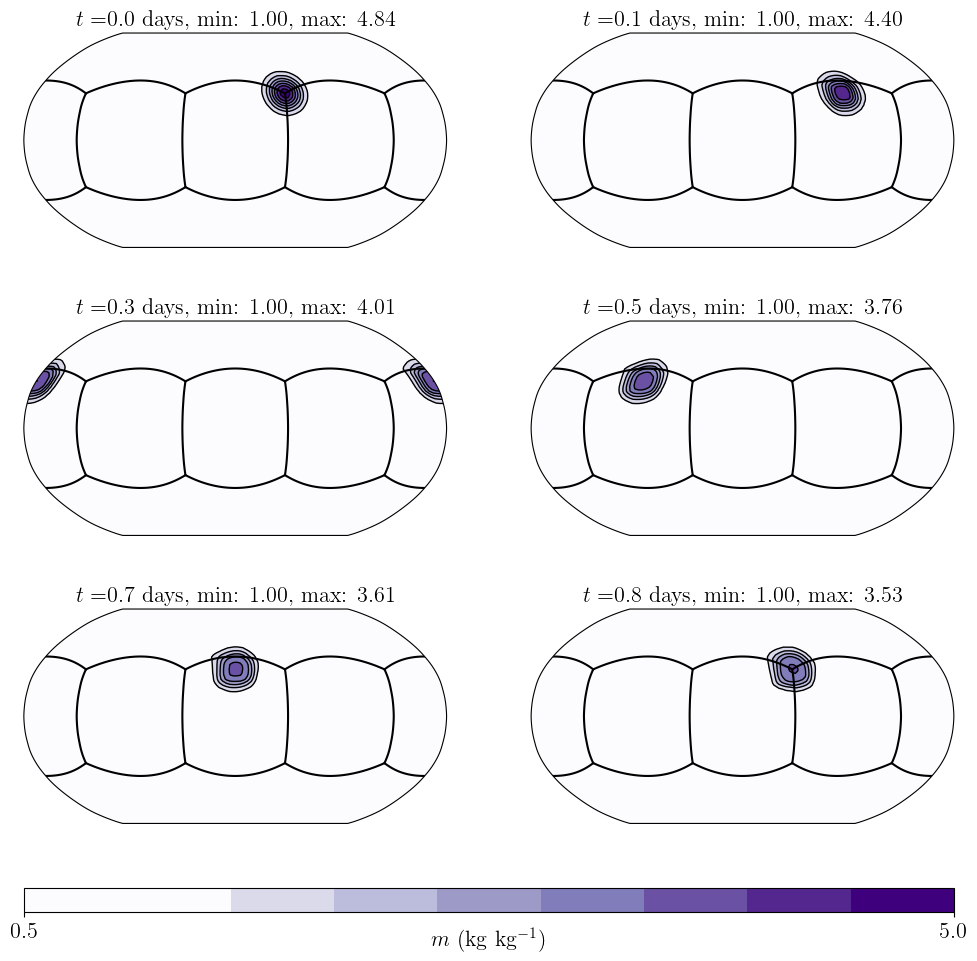
\includegraphics[width=\textwidth]{swift_sbr.png}
    \caption{The transport of a tracer on a cubed-sphere mesh using SWIFT, with only zonal flow to create a solid-body rotation around the pole. The panel edges of the cubed-sphere mesh are included.
    The solution is diffusive as the mesh used has a rather coarse resolution.}
    \label{sbr}
\end{figure}
\\
Our intention is to immediately follow up on this paper with another which demonstrates the application of SWIFT to the cubed-sphere, and we will include results like these there. It might also reassure the reviewer to know that we are currently using the scheme in NWP and climate assessments in the Met Office's new LFRic model, where it is performing well (and without seeing issues like those described by the reviewer!). In any case, we have added some explanation to the text in Section 2a to help clarify this point.
\\
\\
\begin{enumerate}[leftmargin=*]
\item[1.] \textit{On page 15, line 313, the departure point calculations are in part 2 of section 2a.} \\
\\
\textbf{Response}: We have made this change.

\item[2.] \textit{On page 25, section 3d(3), the stability analysis for density requires a constant velocity field, whereupon SWIFT is equivalent to COSMIC.  Stability for tracer transport also requires a constant density field.  However, these restrictions seem rather severe.  Is there any result that could apply with a constant velocity but nonconstant density?  In particular, the case of a density step function $[(u,v) = (1,1)$, $\rho(x>0, y>0) = 1$, else $\rho=0.1$, $\Delta x=\Delta y=\Delta t=1]$ would at least see wildly different Courant numbers in the terms of equation (40), although I'm not sure if this would lead to an instability.  Is there a secondary Lipschitz condition relating to mass fluxes rather than volume fluxes (velocities)?} \\
\\
\textbf{Response}: Traditional stability analysis requires that the scheme is linear, hence the constant velocity and constant density for the analysis. We have tested SWIFT with a variety of different flows, varying density, and Courant numbers (this testing has taken place with the Met Office model) and found that the stability of the scheme does agree with the analysis -- it depends on the Lipschitz condition. The reason for this dependence on Lipschitz is that a Lipschitz number of greater than one means that all of the mass has been removed from a cell during a directional sweep. If the mass is zero (or negative) then the scheme breaks down and becomes unstable. 

\end{enumerate}

\subsection*{Responses to Referee 2}
\underline{Major}
\begin{enumerate}[leftmargin=*]
\item[1.] \textit{Owing to the complexity of the method, the narrative in Sections 2 and 3 will necessarily be challenging. I found that making my own outline was very helpful in following it, but there are places where the notation is changed and there is a lot of unnecessary repetition in definitions.
For example, (18) and (19) are identical to (22), just with different arguments, while the operator $A^x$ in (20a) is called in (16); later in (19) $F^x$ is re-defined based on the additional argument needed for the transport of tracers. I might suggest defining the 1D operators with a consistent notation throughout and then using consistent notation when using these in the 2D schemes.} \\
\\
\textbf{Response}: Thank you for raising these issues. This point was also raised by Referee 1 but we repeat the response here. We have made two significant changes to address this:
\begin{itemize}
    \item The flux operator $\mathcal{F}$ now always has three arguments, so that it is $\mathcal{F}(\rho,u,V)$ for density transport and $\mathcal{F}(m,F,\rho V)$ for conservative tracer transport.
    \item We now use the same equations for both the transport of $\rho$ and $m$ to describe the calculation of departure distances and flux integrals. This allowed the removal of the flux $G$ and several other equations, which we think simplifies the manuscript.
\end{itemize}

\item[2.] \textit{The principal innovations in SWIFT are the introduction of the “unity” field $\sigma$ which essentially corrects an inconsistency in the advection of the density and tracer fields; and the introduction of an additional term in the 1D inner-operator fluxes compared with the Lin-Rood/COSMIC, as shown in (54). Is my understanding correct? Also, am I correct in understanding that the unity field does not need to be preserved between timesteps and is just initialized to be 1 at the start of each new timestep, and that the unity field is only needed for density transport and not for the tracers? (If so, then this makes SWIFT only marginally more expensive than Lin-Rood/COSMIC, mostly requiring the advection of the one additional unity field regardless of the number of tracers, and adding an extra step to the flux evaluations.)} \\
\\
\textbf{Response}: Yes we think your understanding is correct, the additions to the Lin-Rood/COSMIC scheme are principally (a) the difference to the horizontal splitting, and (b) the recomputation of departure points, as volume/mass depends on transported unity/rho. We now compare the two schemes side-by-side in Section 3(d) part 3, and are hoping that this helps to clarify the difference. \\
\\
Yes, the unity field is reset between time steps. The ``transport'' of the unity field is actually very cheap, as it simply involves evaluating the divergence of the wind in the different directions, and so doesn't require parallel communications. However the additional computation of departure points adds extra expense to SWIFT relative to the Lin-Rood/COSMIC scheme, although if multiple tracers are transported then this cost reduces in impact.

\item[3.] \textit{I also didn’t understand the distinction between ``consistency'' and ``constancy'' in this paper: the
latter is obvious (maintenance of a uniform density field or mixing ratio field) but am I correct that
consistency means that constancy of both density and mixing ratio are preserved?} \\
\\
\textbf{Response}: There definitely is an inconsistency in the use of the ``consistency'' in the literature! We have attempted to clarify this in the text, and have also now removed the term ``constancy''. \\
\\
By ``consistency'', we mean that the density of a tracer evolves consistently with the density of dry air, so that any constant mixing ratios are preserved. So this is a property related to tracer transport. \\
\\
The other similar property is what we now call ``divergence-linearity'', that increments to density fields should be linear in $\bm{\nabla\cdot u}$ if the density is constant. The corollary of this is that a constant density will remain so if the flow is divergence-free. We have clarified this in the text and demonstrated that the scheme has this property. \\
\\
We also note that Lin and Rood describe both of these properties as sub-properties of ``consistency'', while Leonard et al discuss only the second (which they describe as ``constancy'').

\item[4.] \textit{The results clearly show that at large Courant numbers SWIFT is more accurate than the older scheme and that it is truly monotonic. One potential advantage that the authors might be missing is that a large Courant number can in some cases be more accurate than a smaller one due to the smaller number of (diffusing) timesteps needed to reach the solution. This is clear from the three tables in Section 4, at least for tracer advection rather than density; and in most cases SWIFT has a larger reduction in error with the larger Courant number than does COSMIC. Do the authors wish to comment on this?} \\
\\
\textbf{Response}: Yes you're right about that, and we've noted it too. For non-uniform flows, the splitting error will still increase with Courant number. We are going to follow up this work with a paper analysing SWIFT applied to spherical domains, and our intention is to assess that error more thoroughly there.

\item[5.] \textit{It was somewhat surprising to me to see a full third-order convergence rate for constant velocity and density fields (Table 4) since I had thought that this sort of splitting method only canceled out the leading-order splitting error. I do notice that sinusoidal initial tracer fields are used for the convergence tests of Section 4.d and not the slotted cylinders used in other parts of Section 4. Is this because we don’t expect a discontinuous solution to converge?} \\
\\
\textbf{Response}: The splitting error of Lin-Rood/COSMIC/SWIFT is second order in time if the velocity is non-constant. For a constant velocity, the splitting error cancels and we obtain the convergence rate of the underlying one-dimensional scheme. We use a sinusoidal tracer for convergence plots as the theoretical spatial order of accuracy of a scheme only holds if the transported field is differentiable up to that order. Hence we would not see the theoretical order of accuracy if measuring the errors for the discontinuous cylinder profile.

\item[6.] \textit{Finally, do the authors have any timing information for SWIFT vs. Lin-Rood/COSMIC?} \\
\\
\textbf{Response}: It's actually not that easy to perform a fair test between the two schemes! For the set-up used for the results presented in the paper, the two schemes are very close in cost (with SWIFT there is just the additional computation of departure points). \\
\\
However, there are alternative formulations using the Lin-Rood/COSMIC splitting that can reduce computational expense -- for instance by using advective operators (e.g.\ standard Semi-Lagragian) for the inner steps of the splitting which can be cheaper than flux calculations. A cheaper lower-order operator can also be used for the inner steps. Neither of these options is possible with the SWIFT splitting. \\
\\
However when monotonicity or positivity is required for steps with large Courant number, SWIFT doesn't require expensive and complicated methods which may be necessary with the Lin-Rood / COSMIC splitting. In LFRic we have found that this benefit outweighed the savings that we could make with the Lin-Rood/COSMIC splitting.
\end{enumerate}

\underline{Minor}
\begin{enumerate}[leftmargin=*]
\item[1.] \textit{Section 2.a.1: One of the advantages of Lin-Rood/COSMIC is that it works with any 1D flux-form operator regardless of subgrid reconstruction. Should this still be true for SWIFT?} \\
\\
\textbf{Response}: Yes, it is still true for the SWIFT splitting that any flux-form 1D scheme can be used (we have tested with Nirvana, piecewise-constant, and Lax-Wendroff schemes). We have clarified this in the paper. However, we wanted to show SWIFT with the most commonly used FFSL type scheme (PPM) which is also under consideration to be used in the Met Office model. We are also planning on expanding on this point in our follow up paper.

\item[2.] \textit{Section 2.a.4, equation (16), and elsewhere: the del operator ($\nabla_x$) typically means a continuous vector derivative of some sort. Is this meant to be a discrete difference in this
manuscript?} \\
\\
\textbf{Response}: Yes, this is meant to represent the (one-dimensional) discrete diveregence calculation. We have updated the text to clarify this.

\item[3.] \textit{Section 2.c.1: Equation (25) should be compared to (14) and not (15), which is more appropriately analogous to (28).} \\
\\
\textbf{Response}: As we have reorganised this section, we believe that this has been resolved.

\end{enumerate}

\subsection*{Responses to Referee 3}
\begin{enumerate}[leftmargin=*]
\item[1.] \textit{In the first paragraph of the introduction, I view (1a) and (2) as the equations that are derived from first principals, at least in all derivations of the NS or Euler equations I have seen, and (1b) is a result of combining (1) and (2). Indeed, it is combining discrete versions of (2) and (1a) to derive an advective-form operator(first appearing in (18)) that is the basis of most of the work in this paper, so perhaps switching (1b) and (2), along with some of the language, is more appropriate for this paper.} \\
\\
\textbf{Response}: We appreciate the reviewer's comment, but having discussed this point with our colleagues we have decided to keep it in the current form. From an atmospheric transport point of view, it is common to solve for density (1a) and for the mixing ratio of a tracer (1b), hence we have kept these in the same equation. It is a key aspect of our work to solve for a mixing ratio using the conservative form, but being consistent with the advective form.

\item[2.] \textit{For readers, understanding equation (18) is critical for understanding the schemes described by the authors in the rest of the paper. The language in the last two sentences in the paragraph preceding equation
(18) need to be formally correct and clear. The current sentences are: \\
\\
``Dividing the conservative transport of $\sigma m$ by the conservative transport of $\sigma$ gives the advective transport
of $m$. This means that advective transport of m in the x-direction is given by''. \\
\\
The phrases conservative transport and advective transport, and the advective transport of $m$, are vague terms. The authors should consider replacing these sentences with: \\
\\
``Dividing the discrete conservative transport update of $\sigma m$ by the discrete conservative transport update of $\sigma$ gives a discrete advective transport update of $m$. This means that the discrete advective transport update of $m$ in the x-direction is given by''} \\
\\
\textbf{Response}: Thank you for the suggestion, we have made this change to improve the clarity of the sentences.

\item[3.] \textit{Line 296: The phrase ``advective form increment'' - the advective form of what? The equation for the evolution of density (1a) is not in advective form. One can write the equation as}
\begin{equation}
 \rho_t = -u\cdot\nabla\rho - \rho\nabla\cdot u   
\end{equation}
\textit{and then one possible correct phrase would be ``the increment from the advection of $\rho$ by the velocity'', i.e.
the first term on the RHS of R1.}
\\
\\
\textbf{Response}: We have been following the terminology used by the Lin \& Rood (1996) paper here but have clarified that an advective operator corresponds to discretising the $\bm{u\cdot\nabla}\rho$ term. 


\item[4.] \textit{What is the point of the section c. SWIFT Splitting for Advective Tracers starting at line 417? I do not see why anyone would want to do this. Perhaps you can remove this section and take the last line of this section and place it at the end of Section 3b?} \\
\\
\textbf{Response}: We have included this because it is used in the current configuration of GungHo (the Met Office's new dynamical core). Although we are going to elaborate on this in future papers, GungHo uses advective-form transport for the wind field and some other tracers. The key distinction is that the advective form is not coupled to the density transport -- and we find that doing this for the transport of wind components is unstable due to our C-grid staggering. However we agree that there is a strong argument for using a standard Semi-Lagrangian scheme instead of using a Flux-Form Semi-Lagrangian scheme. But as this is part of the current configuration that will be in use, we'd like to keep it in the paper.

\item[5.] \textit{Last paragraph of section 3, concerning Strang splitting: If one is willing to do some extra work, symmetry is not difficult to obtain in a Strang split scheme. Skamarock (2006) suggested a 3D splitting $x$-$y$-$z$ followed on the next step by $z$-$y$-$x$. A symmetric scheme in $x, y)$ for a timestep could average
an $x$-$y$ split with a $y$-$x$ split, and then proceed to $z$. Regarding the halo exchanges, only half as much data needs to get passed at any one time in the standard splitting because of the splitting. Although one could compute in one direction out in the halo to provide data for the next pass in the other direction if the computations are faster. My guess is that a symmetric Strang split scheme would be competitive with the SWIFT scheme.} \\
\\
\textbf{Response}: This is an interesting idea. The starting point of our work was the Lin-Rood/COSMIC splitting and how to make it monotonic in 2D, and then how to use it and keep it monotonic in 3D without excessive cost. The Strang splitting you suggest is one we may look at as a comparison to SWIFT in our follow-up paper that focuses on the sphere.

\item[6.] \textit{Section 4a, Constant Velocity Test: Do the 128x128 cells cover the -0.5,+0.5 domain? Perhaps stated differently, are we seeing the entire domain in the plots in Figure 2?} \\
\\
\textbf{Response}: Yes it covers the whole domain and we see this in the plots. The domain is size 1000 m, from -0.5 km to 0.5 km, and is periodic. We have clarified this in the text. There was an error in the text relating to the time used in some of the tests and this has been corrected.

\item[7.] \textit{Should I assume the lateral boundary conditions are double periodic, and the slotted cylinders shown in Figure 2 have returned to their starting locations at the end of the integration?} \\
\\
\textbf{Response}: Yes, we have clarified this in the text.

\item[8.] \textit{The slotted cylinder results for the COSMIC scheme shown in the upper-center and upper right panels in Figure 2 show slotted cylinders that are very different in their errors (the right cylinders look much
worse than the left ones). Do we know why that is the case?} \\
\\
\textbf{Response}: The difference between the centre and right hand plots is that the centre plots are without monotonicity, and the right plots are with monotonicity. The monotonic limiters introduce diffusion to the solution, and hence without monotonicity there are much larger magnitude errors and oscillations.

The difference between the left and right tracers (in the centre top plot) for COSMIC is due to the asymmetry introduced by the non-constant density. This can be seen more clearly in Figure 4 where the two tracers undergo different motion during the flow. At large Courant numbers the COSMIC scheme produces very large overshoots and undershoots, which SWIFT does not.

\item[9.] \textit{Section 5b, shifted grid for the Charney-Phillips vertical staggering: Do the small cells on the top and bottom of the shifted grid affect the stability (e.g. producing a larger Lipschitz number).} \\
\\
\textbf{Response}: {Yes, the small cells could impact the stability as they have smaller depth, although we have not found this to be a particular issue in the dynamical core (which also enforces zero normal wind at the top and bottom boundaries of the domain).

\end{enumerate}


\end{document}